% Deployment view: every container in docker-compose.yml, the topics, and who writes and reads them.
\documentclass[tikz,border=4pt]{standalone}
\usepackage[T1]{fontenc}
\usepackage{lmodern}
\usetikzlibrary{positioning,fit,arrows.meta,calc,backgrounds}
% Shared look for every diagram. \input this after \usetikzlibrary.
% Greys plus one accent, so the figures print fine in black and white.
\definecolor{accent}{HTML}{2563EB}
\definecolor{accentlight}{HTML}{DBEAFE}
\definecolor{latecol}{HTML}{B45309}
\definecolor{latelight}{HTML}{FEF3C7}
\definecolor{grey}{HTML}{6B7280}
\definecolor{greylight}{HTML}{F3F4F6}
\tikzset{
  box/.style={draw, rounded corners=2pt, align=center, minimum height=7mm, inner sep=3pt, fill=white, font=\footnotesize},
  topic/.style={box, fill=greylight, draw=grey},
  op/.style={box, draw=accent, fill=accentlight},
  ctr/.style={draw=grey, dashed, rounded corners=4pt, inner sep=3mm},
  note/.style={font=\scriptsize, text=grey, align=left},
  arr/.style={-{Latex[length=2mm]}, thick},
  shuffle/.style={arr, double, double distance=0.6pt, -{Latex[length=2.4mm]}},
  latearr/.style={arr, dashed, draw=latecol},
  lbl/.style={font=\scriptsize, fill=white, inner sep=1pt},
}

\begin{document}
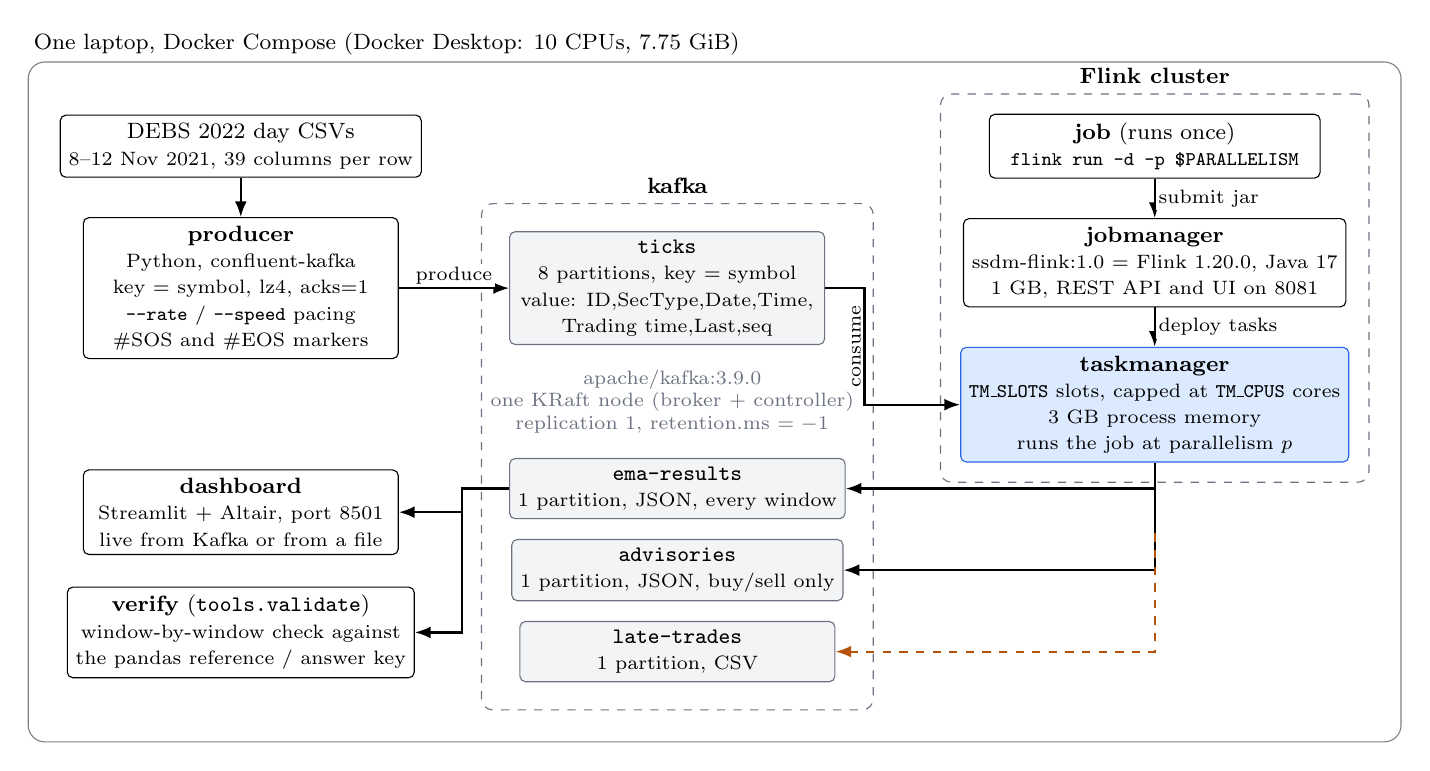
\begin{tikzpicture}[node distance=6mm and 9mm]
  % ---- column 1: input and consumers
  \node[box, minimum width=40mm] (csv) {DEBS 2022 day CSVs\\\scriptsize 8--12 Nov 2021, 39 columns per row};
  \node[box, below=5mm of csv, minimum width=40mm] (prod) {\textbf{producer}\\\scriptsize Python, confluent-kafka\\\scriptsize key = symbol, lz4, acks=1\\\scriptsize \texttt{-{}-rate} / \texttt{-{}-speed} pacing\\\scriptsize \#SOS and \#EOS markers};
  \node[box, below=14mm of prod, minimum width=40mm] (dash) {\textbf{dashboard}\\\scriptsize Streamlit + Altair, port 8501\\\scriptsize live from Kafka or from a file};
  \node[box, below=4mm of dash, minimum width=40mm] (val) {\textbf{verify} (\texttt{tools.validate})\\\scriptsize window-by-window check against\\\scriptsize the pandas reference / answer key};
  % ---- column 2: kafka
  \node[topic, right=14mm of prod, minimum width=40mm] (ticks) {\texttt{ticks}\\\scriptsize 8 partitions, key = symbol\\\scriptsize value: ID,SecType,Date,Time,\\\scriptsize Trading time,Last,seq};
  \node[topic, right=14mm of dash, minimum width=40mm, yshift=3mm] (res) {\texttt{ema-results}\\\scriptsize 1 partition, JSON, every window};
  \node[topic, below=2.5mm of res, minimum width=40mm] (adv) {\texttt{advisories}\\\scriptsize 1 partition, JSON, buy/sell only};
  \node[topic, below=2.5mm of adv, minimum width=40mm] (late) {\texttt{late-trades}\\\scriptsize 1 partition, CSV};
  \begin{scope}[on background layer]
    \node[ctr, fit=(ticks)(res)(adv)(late), inner sep=3.5mm, label={[font=\footnotesize\bfseries]north:kafka}] (kafka) {};
  \end{scope}
  \node[note, align=center] at ($(ticks.south)!0.5!(res.north)$) {apache/kafka:3.9.0\\one KRaft node (broker + controller)\\replication 1, retention.ms $=-1$};
  % ---- column 3: flink
  \node[box, right=14mm of csv, xshift=58mm, minimum width=42mm] (job) {\textbf{job} (runs once)\\\scriptsize \texttt{flink run -d -p \$PARALLELISM}};
  \node[box, below=5mm of job, minimum width=42mm] (jm) {\textbf{jobmanager}\\\scriptsize ssdm-flink:1.0 = Flink 1.20.0, Java 17\\\scriptsize 1 GB, REST API and UI on 8081};
  \node[op, below=5mm of jm, minimum width=42mm] (tm) {\textbf{taskmanager}\\\scriptsize \texttt{TM\_SLOTS} slots, capped at \texttt{TM\_CPUS} cores\\\scriptsize 3 GB process memory\\\scriptsize runs the job at parallelism $p$};
  \begin{scope}[on background layer]
    \node[ctr, fit=(job)(jm)(tm), inner sep=2.5mm, label={[font=\footnotesize\bfseries]north:Flink cluster}] (flink) {};
  \end{scope}
  % ---- arrows
  \draw[arr] (csv) -- (prod);
  \draw[arr] (prod) -- node[lbl, above]{produce} (ticks);
  \draw[arr] (job) -- node[lbl, right]{submit jar} (jm);
  \draw[arr] (jm) -- node[lbl, right]{deploy tasks} (tm);
  \draw[arr] (ticks.east) -- ++(5mm,0) |- node[lbl, pos=0.25, fill=none, rotate=90, above]{consume} (tm.west);
  \coordinate (fan) at ($(tm.south)+(0,-9mm)$);
  \draw[thick] (tm.south) -- (fan);
  \draw[arr] (fan) |- (res.east);
  \draw[arr] (fan) |- (adv.east);
  \draw[latearr] (fan) |- (late.east);
  \draw[arr] (res.west) -- ++(-6mm,0) |- (dash.east);
  \draw[arr] (res.west) -- ++(-6mm,0) |- (val.east);
  % ---- the host
  \begin{scope}[on background layer]
    \node[draw=black!50, rounded corners=6pt, inner sep=4mm, fit=(csv)(val)(kafka)(flink),
          label={[font=\footnotesize, anchor=south west, inner sep=2pt]north west:One laptop, Docker Compose (Docker Desktop: 10 CPUs, 7.75 GiB)}] {};
  \end{scope}
\end{tikzpicture}
\end{document}
